\section{Methods}
\label{sec:methods}

%==========================================================================
% TODO: PÁRRAFO INICIAL - Resumen de la sección
%==========================================================================
% [AQUÍ FALTA: Un párrafo breve (2-3 oraciones) que resuma la estrategia
% metodológica y anticipe las subsecciones. En NeurIPS esto ayuda al revisor.
%
We implemented a large-scale spiking neural network using the NEST simulator \citep{Gewaltig2007}. We constructed three architectural configurations of increasing complexity, all grounded in the canonical cortical microcircuit \citep{Potjans2014}: (1) V1 columns with only lateral intra-areal connections, (2) a V1-V2 hierarchy with simple convergent feedback, and (3) a V1-V2 hierarchy with reciprocal lateral inhibition between V2 modules. In the following sections we describe the neuron model, the laminar microcircuit architecture, the hierarchical connectivity, the stimulation protocols, and the data analysis pipeline.

%==========================================================================
% \subsection{Neuron Model and Simulation Environment}
%==========================================================================
\textbf{3.1 Neuron Model and Simulation Environment.} Neurons were modeled as leaky integrate-and-fire (LIF) units with exponential-decaying postsynaptic currents. The subthreshold membrane potential dynamics are governed by the membrane time constant ($\tau_m = 10$ ms), membrane capacity ($C_m = 250$ pF), and resting potential ($V_{\text{rest}} = -65$ mV). A spike is emitted when $V_m$ reaches the threshold ($V_{\text{th}} = -50$ mV), after which the potential is clamped to the reset value ($V_{\text{reset}} = -65$ mV) for an absolute refractory period ($\tau_{\text{ref}} = 2$ ms). Excitatory synaptic weights were set to $w = 87.8 \pm 8.8$ pA with a decay time constant $\tau_{\text{syn}} = 0.5$ ms, and relative inhibitory synaptic strength was fixed at $g = -4$. Transmission delays were drawn from uniform distributions of $1.5 \pm 0.75$ ms for excitatory synapses and $0.75 \pm 0.38$ ms for inhibitory synapses. Background cortical activity was emulated via Poisson spike trains delivered to all neurons at a mean rate of $8$ Hz. All parameters were tuned to sustain the asynchronous-irregular firing regime characteristic of awake cortical states. Simulations were performed using the NEST simulator \citep{Gewaltig2007}.
%==========================================================================
% TODO: ECUACIÓN DEL LIF
%==========================================================================
% [AQUÍ FALTA: Incluir la ecuación del potencial de membrana del LIF. Tienes
% dos opciones:
%   - Opción A (ecuación diferencial):
%     \tau_m \frac{dV_m}{dt} = -(V_m - V_{rest}) + R_m I(t)
%   - Opción B (formulación de conductancia con corrientes sinápticas):
%     \tau_m \frac{dV_m}{dt} = -(V_m - V_{rest}) + \sum_{j} w_j e^{-t/\tau_{syn}}
%
The membrane potential evolves according to
\begin{equation}
  \tau_m \frac{dV_m}{dt} = -(V_m - V_{\text{rest}}) + R_m I_{\text{syn}}(t),
\end{equation}
where $R_m$ is the membrane resistance and $I_{\text{syn}}(t)$ is the total synaptic current. Each synaptic input generates a conductance-based current with exponential decay,
\begin{equation}
  I_{\text{syn}}(t) = w \, e^{-t / \tau_{\text{syn}}},
\end{equation}
where $w$ is the synaptic weight and $\tau_{\text{syn}}$ is the synaptic time constant.

%==========================================================================
% \subsection{Laminar Microcircuit Architecture}
%==========================================================================
\textbf{3.2 Laminar Microcircuit Architecture.} Each V1 module represents a $1$ mm$^2$ patch of cortical tissue, based on the full-scale canonical microcircuit model proposed by \citet{Potjans2014}. It comprises approximately $77{,}000$ neurons distributed across four laminar layers: L2/3, L4, L5, and L6. Within each layer, the network maintains a physiological ratio of excitatory to inhibitory neurons of approximately 80/20. Local recurrent connectivity follows empirically derived connection probabilities.

To capture intra-areal spatial integration, long-range horizontal projections within V1 are incorporated. These lateral connections are restricted to the superficial L2/3 layer and are functionally segregated by distance. Nearby connections link functionally similar adjacent columns with both excitatory and inhibitory synapses, with transmission delays of $d_{\text{n.lat}} = 5 \pm 1.5$ ms. Distant connections, in contrast, link columns with disparate orientation preferences and operate via a predominantly suppressive mechanism through disynaptic inhibition, with a slower conduction delay of $d_{\text{d.lat}} = 8 \pm 2.5$ ms.

%==========================================================================
% TODO: TABLA DE CONEXIONES O FIGURA DEL MICROCIRCUITO
%==========================================================================
% [AQUÍ FALTA: Referenciar una tabla o figura que resuma las probabilidades
% de conexión entre poblaciones. Si no quieres incluir la tabla completa de
% Potjans & Diesmann, al menos menciona que usas las mismas probabilidades y
% remite a una tabla en el apéndice.
%
\commentcd{Aca se habla del apéndice }The complete connection probability matrix between the eight neuronal populations (four layers $\times$ two types) follows the values reported by \citet{Potjans2014} and is provided in Table~\ref{tab:connectivity} of the Appendix.

\begin{figure}[t]
  \centering
  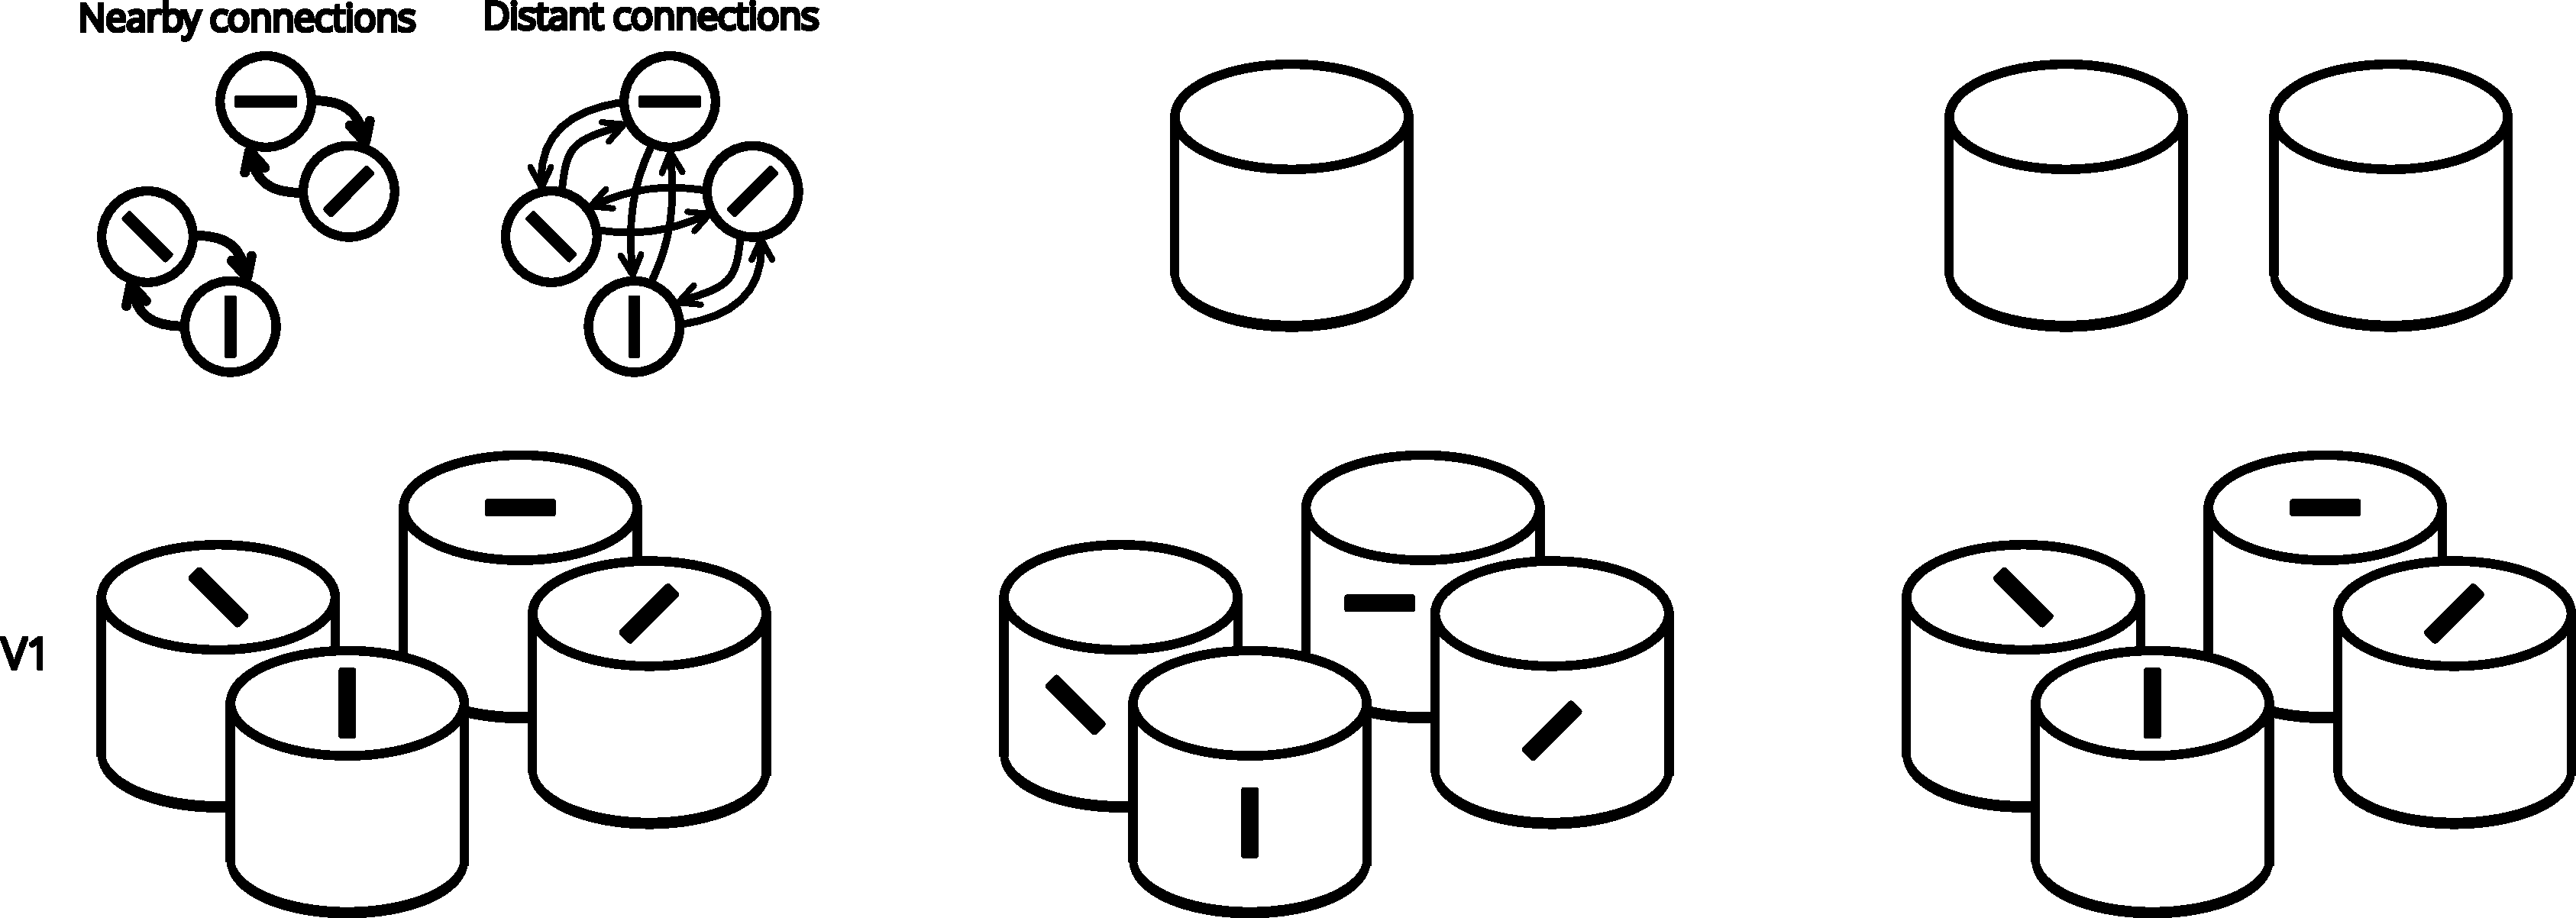
\includegraphics[width=\textwidth]{img/architectures.pdf}
  \caption{%
    \textbf{Architectural configurations compared in this study.}
    \textbf{(A)} Connections of the canonical V1 circuit.
    \textbf{(B)} Overall architecture of the near and distant lateral connections, and the feedforward and feedback connections between V1 and V2.
    \textbf{(C)} Configuration~1: V1 microcolumns with lateral intra-areal connections only.
    \textbf{(D)} Configuration~2: V1-V2 hierarchy with a single V2 module providing non-specific feedback.
    \textbf{(E)} Configuration~3: V1-V2 hierarchy with two V2 modules interconnected via reciprocal lateral inhibitory connections, implementing hierarchical winner-take-all competition.
  }
  \label{fig:architectures}
\end{figure}

%==========================================================================
% \subsection{Hierarchical Integration and Competitive Dynamics}
%==========================================================================
\textbf{3.3 Hierarchical Integration and Competitive Dynamics.} To investigate the mechanistic origins of eCRF effects, the baseline architecture was extended to include a higher-order visual area (V2). The V2 module mirrors the cytoarchitectural variations in laminar thickness and neuronal densities reported for the macaque V2 region. Inter-areal communication is mediated by topographic projections with fast transmission delays of $2 \pm 0.5$ ms. Feedforward pathways originate from the superficial layers L2/3 of V1 and terminate predominantly in L4 and L6 of V2. Feedback projections originate from the deep layers L5 and L6 of V2 and target the superficial L2/3 and infragranular L5 of V1, anatomically avoiding L4 to provide modulatory rather than driving input.

To test the hypothesis that eCRF phenomena emerge from inter-areal interactions rather than purely local filtering, we embedded a lateral competition mechanism within the V2 module. This architecture comprises two spatially distinct, feature-aligned V2 modules that engage in competition via strong, reciprocal inhibitory connections. This hierarchical winner-take-all dynamic non-linearly refines the top-down feedback signals before they modulate V1 activity, overcoming the limitations of linear feedback models and enabling the robust, stimulus-specific surround suppression observed in physiological recordings.

%==========================================================================
% TODO: DESCRIPCIÓN FORMAL DE LAS TRES ARQUITECTURAS
%==========================================================================
% [AQUÍ FALTA: Describir explícitamente las tres configuraciones que
% comparaste, de forma que quede claro qué tiene cada una y qué no.
%
To isolate the contribution of each circuit component, we systematically compared three architectural configurations (see Figure~\ref{fig:architectures}). \textbf{(1) V1 lateral only:} Four V1 microcolumns arranged in a ring, interconnected exclusively via horizontal connections within L2/3. No V2 modules are present. \textbf{(2) V1 + linear V2 feedback:} The V1 columns project feedforward to a single V2 module, which pools inputs from all columns and returns non-specific feedback to V1. This configuration implements hierarchical feedback without lateral competition. \textbf{(3) V1 + competitive V2 feedback:} The V1 columns project feedforward to two V2 modules, each aligned to a specific orientation column. The two V2 modules are interconnected via strong, reciprocal inhibitory synapses, implementing a winner-take-all competition. All other parameters, including neuron counts, local connectivity, and stimulation protocols, were held constant across configurations to ensure that differences in suppression magnitude can be attributed exclusively to the architectural manipulation.

%==========================================================================
% TODO: FIGURA DE LAS TRES ARQUITECTURAS
%==========================================================================
% [AQUÍ FALTA: Referencia a una figura esquemática mostrando las tres
% configuraciones lado a lado. Esto es crítico para NeurIPS.
%

\begin{figure}[t]
  \centering
  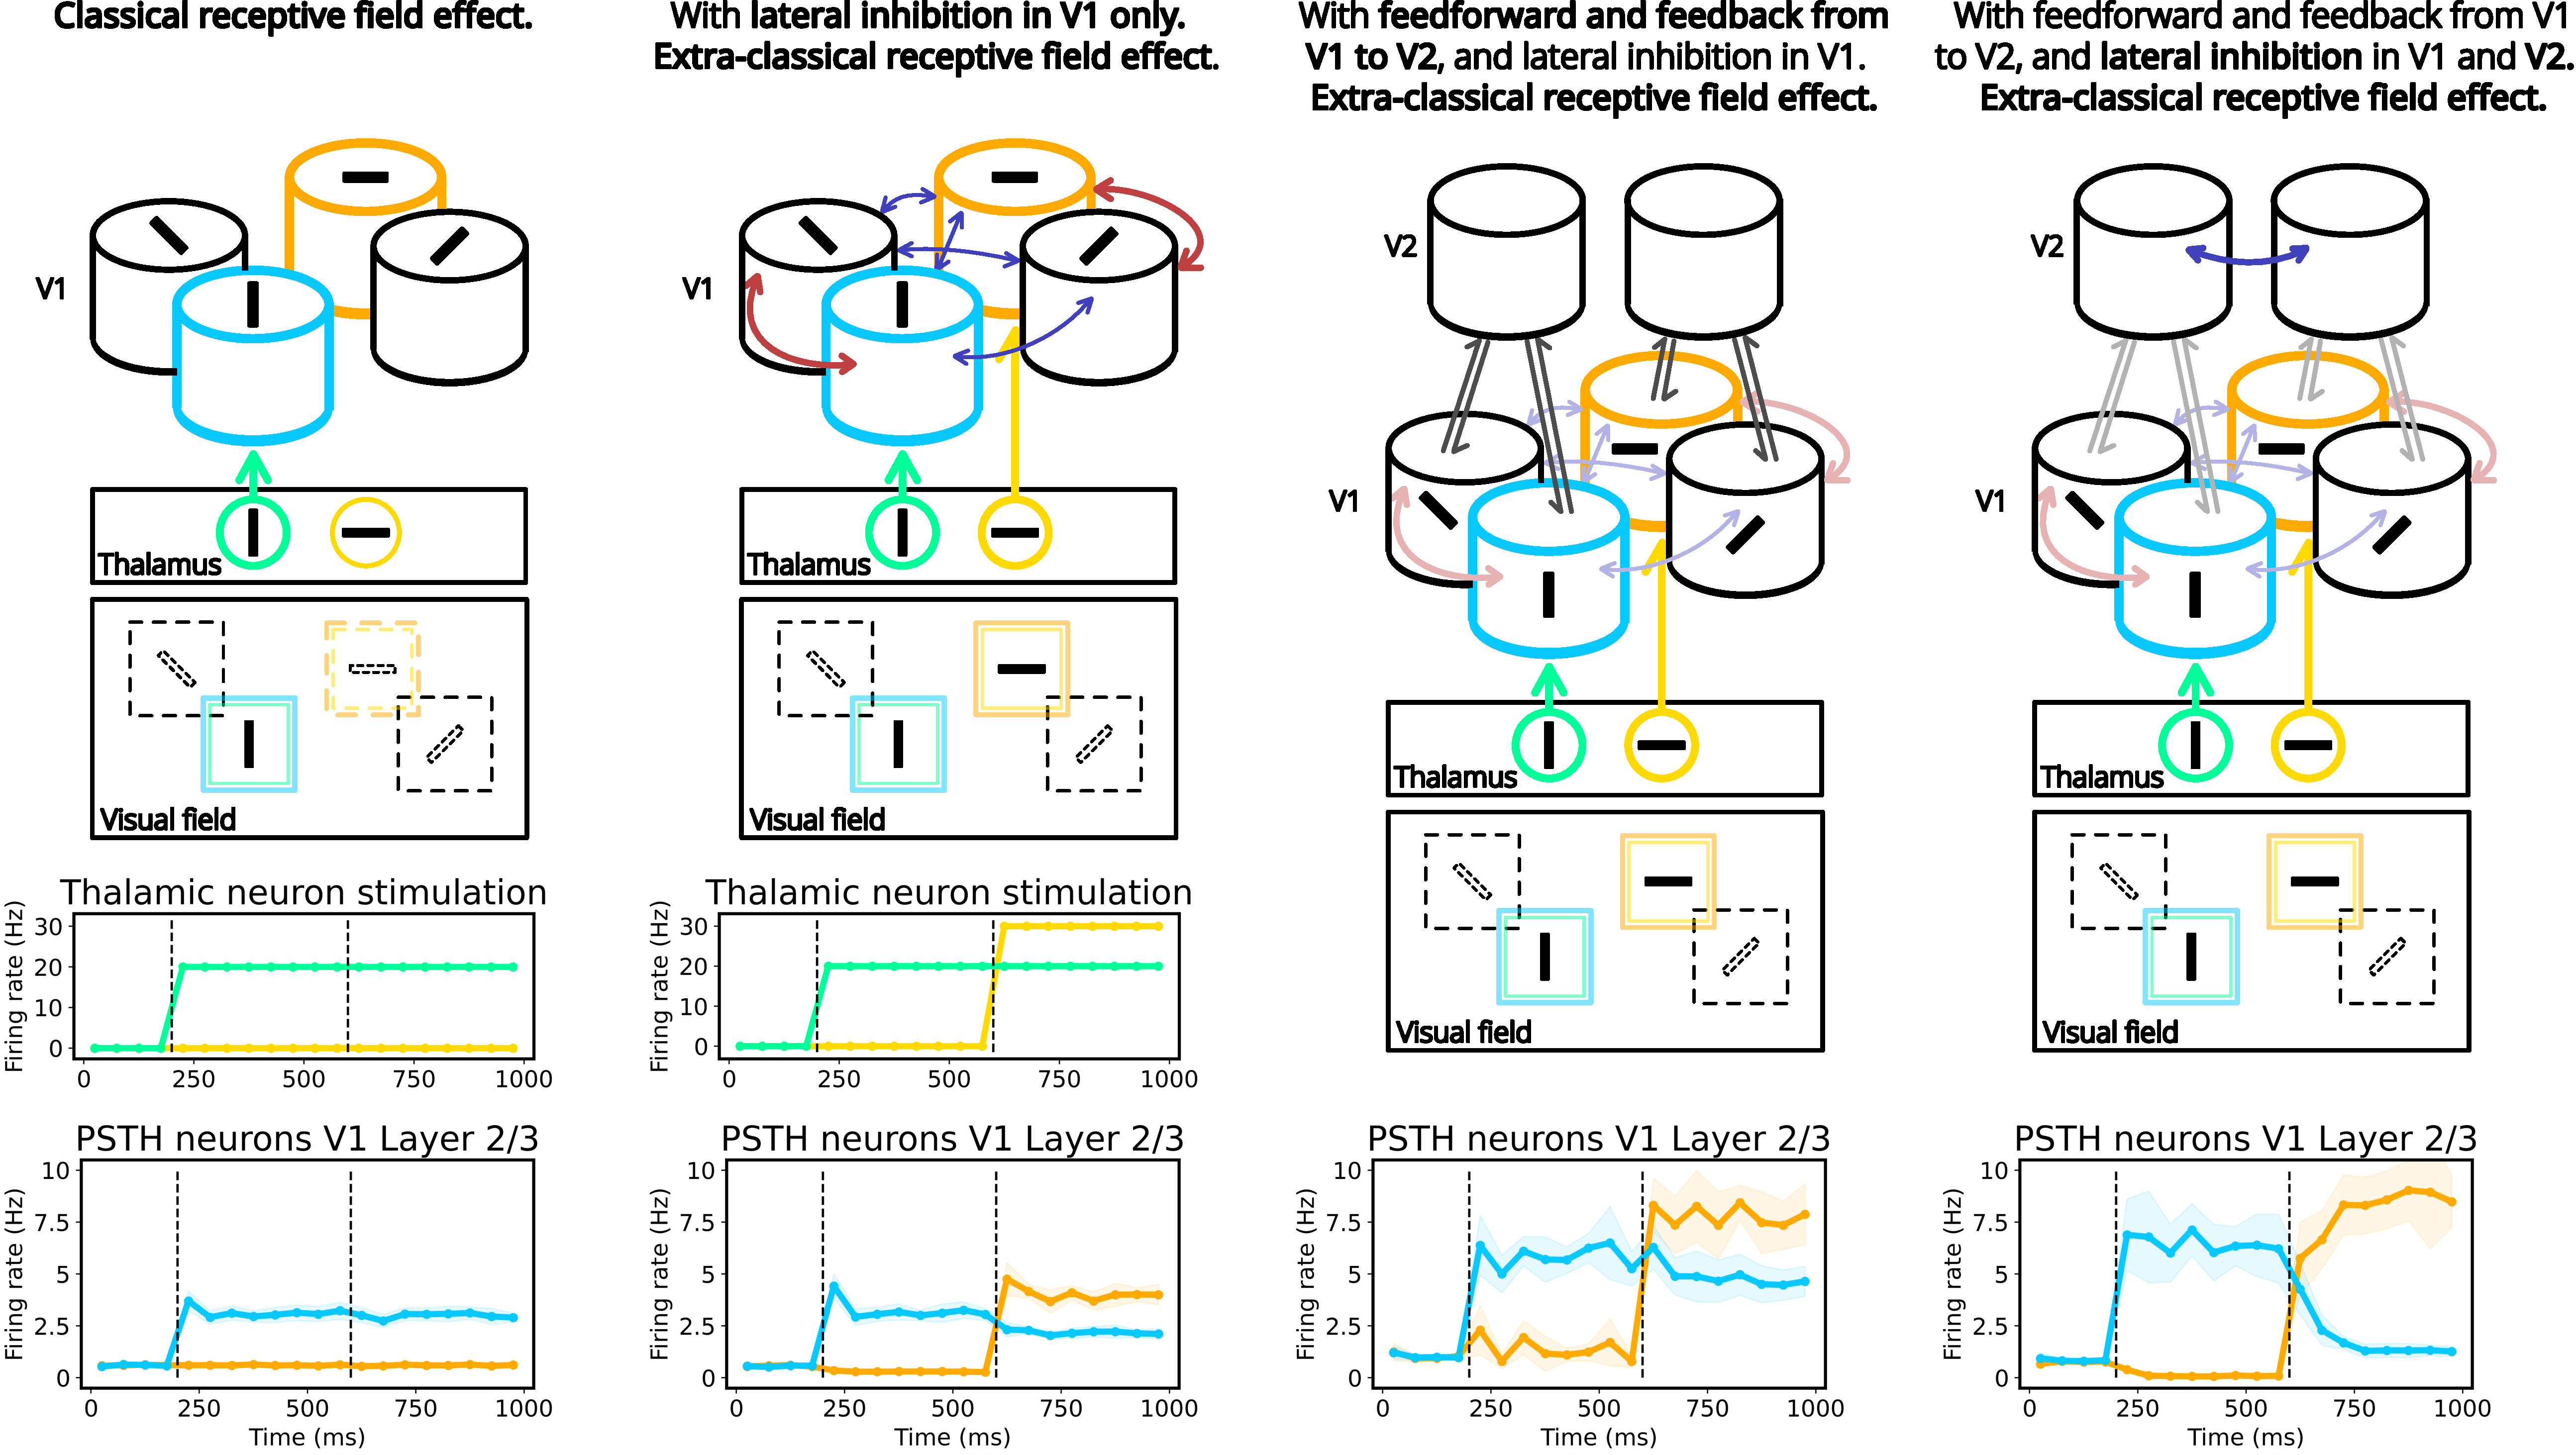
\includegraphics[width=\textwidth]{img/protocol.pdf}
  \caption{%
    \textbf{Architectural configurations compared in this study.}
    \textbf{(A)} Connections of the canonical V1 circuit.
    \textbf{(B)} Overall architecture of the near and distant lateral connections, and the feedforward and feedback connections between V1 and V2.
    \textbf{(C)} Configuration~1: V1 microcolumns with lateral intra-areal connections only.
    \textbf{(D)} Configuration~2: V1-V2 hierarchy with a single V2 module providing non-specific feedback.
    \textbf{(E)} Configuration~3: V1-V2 hierarchy with two V2 modules interconnected via reciprocal lateral inhibitory connections, implementing hierarchical winner-take-all competition.
  }
  \label{fig:architectures}
\end{figure}

%==========================================================================
% \subsection{Sensory Stimulation Protocols}
%==========================================================================
\textbf{3.4 Sensory Stimulation Protocols.} Bottom-up sensory stimulation was emulated via thalamocortical afferents originating from the lateral geniculate nucleus (LGN), projecting primarily to layers L4 and L6 of V1. Thalamic inputs were modeled as Poisson spike trains. To simulate the classical receptive field response, the thalamic firing rate directed at the central microcolumn was increased to $20$ Hz after a $500$ ms baseline period. To evaluate extra-classical modulation, a peripheral contextual stimulus was applied to a distant column at $1000$ ms. The intensity of this peripheral stimulus was systematically varied across three levels: $10$, $20$, and $30$ Hz.

%==========================================================================
% TODO: DEFINICIÓN FORMAL DEL SUPPRESSION INDEX
%==========================================================================
% [AQUÍ FALTA: Definir matemáticamente el índice de supresión. Fundamental
% para que los resultados sean reproducibles.
%
To quantify the strength of surround suppression, we define the suppression index (SI) as
\begin{equation}
  \text{SI} = 1 - \frac{R_{\text{center+surround}}}{R_{\text{center}}},
\end{equation}
where $R_{\text{center}}$ is the mean firing rate of the central column during classical receptive field stimulation alone, and $R_{\text{center+surround}}$ is the mean firing rate during concurrent center and peripheral stimulation. An SI of $1$ indicates complete suppression, and an SI of $0$ indicates no contextual modulation.

%==========================================================================
% \subsection{Data Analysis and Local Field Potentials}
%==========================================================================
\textbf{3.5 Data Analysis.} Network dynamics and mean firing rates were evaluated using peri-stimulus time histograms (PSTH). To connect the spiking network model to macroscopic electrophysiological biomarkers, including gamma-band oscillations and excitation/inhibition balance alterations, we simulated the local field potential (LFP) using a spatiotemporal kernel-based approximation. In this framework, the LFP was reconstructed as the linear superposition of unitary field potentials generated by individual action potentials, enabling spectral analysis of the network rhythmic activity under distinct contextual modulations.

%==========================================================================
% TODO: COMPLEJIDAD COMPUTACIONAL Y RECURSOS
%==========================================================================
% [AQUÍ FALTA: Una frase o dos sobre los recursos computacionales usados.
% En NeurIPS esto es cada vez más esperado.
%
All simulations were executed on a high-performance computing cluster using [X] nodes with [Y] cores and [Z] GB of RAM. A typical simulation of $5$ seconds of biological time for Configuration~3, comprising approximately [N] neurons and [M] synapses, required roughly [T] hours of wall-clock time. The code to reproduce all simulations and analyses will be released upon publication.